\documentclass[twoside,12pt]{article}

\usepackage{mdframed}
\usepackage[hmarginratio=1:1,top=32mm,columnsep=20pt]{geometry} % Document margins
\usepackage{multicol} % Used for the two-column layout of the document
\usepackage[hang, small,labelfont=bf,up,textfont=it,up]{caption} % Custom captions under/above floats in tables or figures
\usepackage{booktabs} % Horizontal rules in tables
\usepackage{float} % Required for tables and figures in the multi-column environment - they need to be placed in specific locations with the [H] (e.g. \begin{table}[H])
\usepackage{hyperref} % For hyperlinks in the PDF
\usepackage{amsmath,amsthm,amssymb}
\usepackage{lettrine} % The lettrine is the first enlarged letter at the beginning of the text
\usepackage{paralist} % Used for the compactitem environment which makes bullet points with less space between them
\usepackage{tikz}
\usepackage{esint}
\usepackage{centernot}
\usepackage{lmodern}
\usetikzlibrary{3d}
\usetikzlibrary{patterns,calc,hobby}
\usetikzlibrary{decorations.pathreplacing}
\tikzset{
	partial ellipse/.style args={#1:#2:#3}{
		insert path={+ (#1:#3) arc (#1:#2:#3)}
	}
}
\usepackage{xcolor}

\usepackage{fancyhdr} % Headers and footers
\pagestyle{fancy} % All pages have headers and footers
\fancyhead{} % Blank out the default header
\fancyfoot{} % Blank out the default footer
\fancyhead[C]{Jimmy Yue $\bullet$ Complex Systems$\bullet$ Jimmy Yue} % Custom header text
\fancyfoot[RO,LE]{\thepage} % Custom footer text

\newmdenv[skipabove=7pt,
rightline=false,
leftline=true,
topline=false,
bottomline=false,
skipbelow=5pt,
linecolor=black,
innerleftmargin=5pt,
innerrightmargin=5pt,
innertopmargin=5pt,
leftmargin=0cm,
rightmargin=0cm,
linewidth=4pt,
innerbottommargin=5pt]{cBox}

\theoremstyle{definition}
\newtheorem*{solutionT}{Solution}

\newenvironment{solution}{\begin{cBox}\begin{solutionT}}{\hfill{\scriptsize\ensuremath{\square}}\end{solutionT}\end{cBox}}

%%%%%%%%%%%%%%%%%%%%%%%%%%%%%%%%%%%%%%%%%%%%%%%%%%%%%%%%%%%%%%%%%%%%%%%%%%%%%%%%%%%%%%%%%%%%
\newcommand{\vect}[1]{\vec{\pmb{#1}}}
\newcommand{\uvect}[1]{\hat{\mathbf{#1}}}
\newcommand{\leviciv}{\epsilon_{ijk}}

\newmdenv[skipabove=7pt,
rightline=false,
leftline=true,
topline=false,
bottomline=false,
skipbelow=5pt,
linecolor=black,
innerleftmargin=5pt,
innerrightmargin=5pt,
innertopmargin=5pt,
leftmargin=0cm,
rightmargin=0cm,
linewidth=4pt,
innerbottommargin=7,
backgroundcolor=light-gray]{dBox}



\theoremstyle{definition}
\newtheorem*{proof1}{Definition}

\newenvironment{ddef}{\begin{dBox}\begin{proof1}}{\hfill{\scriptsize}\end{proof1}\end{dBox}}
\newcommand{\pdif}[2]{\frac{\partial#1}{\partial#2}}
\definecolor{light-gray}{gray}{0.85}
%----------------------------------------------------------------------------------------
%-	TITLE SECTION
%----------------------------------------------------------------------------------------

\title{\vspace{-15mm}\fontsize{24pt}{10pt}\selectfont\textbf{Complex Systems Assignment 1}} % Article title

\author{
\large
\textsc{Jimmy Tsz Ming Yue}\\[2mm] % Your name
\normalsize University of Sydney \\ % Your institution
\normalsize \href{mailto:jyue6728@uni.sydney.edu.au}{jyue6728@uni.sydney.edu.au} % Your email address
\vspace{-5mm}
}
\date{}

%----------------------------------------------------------------------------------------

\usepackage{Sweave}
\begin{document}

\maketitle % Insert title
\setlength{\headheight}{52pt}
\thispagestyle{fancy} % All pages have headers and footers

\abstract{\emph{We review the paper ``An Agent-Based Modelling for Pandemic Influenza in Egypt'' \cite{DBLP:journals/corr/abs-1001-5275} which uses an agent based model to evaluate the pathogenic spread of the H1N1 virus strain. We will both outline the model described and critically evaluate the application of this model to study the complex system of epidemic and pandemic spread. \footnote{The abstract is not meant to be part of the assignment, it merely gives an overview and attempts to frame the assignment to the question. It was not taken into consideration with the word count}}

\begin{multicols}{2}
	\section{Summary} 
	The spread of Influenza strains such as H1N1 is often simulated for control strategies to be implemented. The paper \cite{DBLP:journals/corr/abs-1001-5275} uses agent-based modelling (ABM) to describe social interaction under pandemic situations to develop a model of viral spread as an extension to deterministic SIR models. SIR models generate three separate classes ; Susceptible ($S$), Infected ($I$) and Recovered ($R$) which are linked through a series of coupled differential equations. The authors generate an extension through addition of new states $(C)$, $(E)$, $(NQ)$, $(Q)$, $(D)$, $(M)$, shown: 
	\begin{figure}[H]
	\centering
	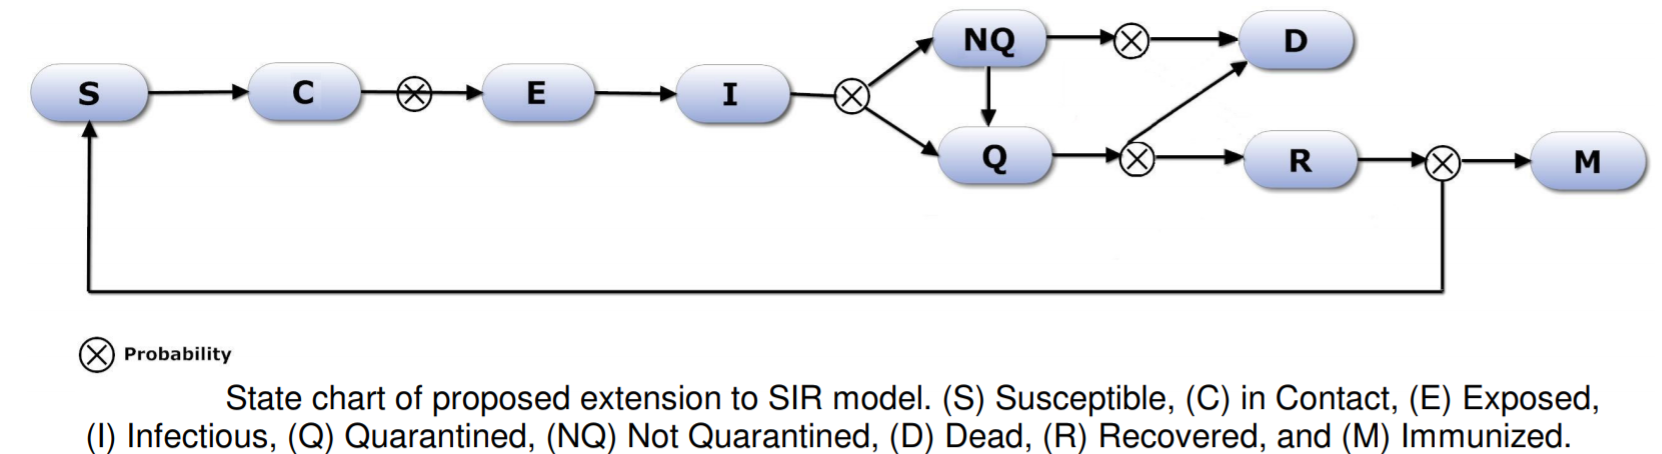
\includegraphics[width=\linewidth]{1.png}
	\caption{Extended SIR states, with directed state evolution. \cite{DBLP:journals/corr/abs-1001-5275}}
	\label{fig1}
	\end{figure}

	for which agent based modelling of social behaviour realistically simulate the evolution of such states. These social behaviour is determined by the social class that agents are classified by, through a reflection of Egypt's census data in 2006. This is done through the population percentage classification of age groups, for which each group possess their own likely interaction networks. Such interactions determine the spread under the extended SIR model, forming the basis of agent based rulesets. Under these ruleset, the agents visit their social networks, such as children visiting schools etc; allowing susceptible agents to undergo state changes outlined in fig. \ref{fig1}, with increased infected agent contact heightening the stochastic process of infection. The model is run in loops over the course of pre-defined simulated days, with agents performing their social interactions. Validation was conducted through comparison of simplified situations against the SIR model, which was found to be closely matched despite smoothness considerations. With this validation, the author(s) placed epidemic control strategies such as immunisation and disease awareness into practice to examine the effects on epidemics.  It was found that under such measures, infected populations were reduced with differing effectiveness, however some treatments such as social distancing and quarantine remained ineffective at epidemic peaks. The authors further conclude that models with higher fidelity to realism such as the addition of gender and other agent parameters may lead to better simulation, and optimal control strategies.\\
	This study was highly effective in capturing basic elements of social interactivity during epidemic situations, with validation showing high fidelity to previous SIR models \cite{Kermack700}, and results reflecting the effectiveness of control strategies. However due to the complexity of the system, there are still many refinements to the underlying extension of the SIR model that may influence any agent based models, along with refinement of agent rulesets through utilising differing demographic classifications instead of age. One such example is social economic statuses as this describes the availablity to medicine and education to understand viral transmission. In summary the study highlights the effectiveness of agent based modelling in providing consideration of social networks in pandemic spread.

		
\end{multicols}
\bibliographystyle{plain}
\bibliography{week1.bib}
\textbf{Word Count (deTeX, without Abstract):} 499\\
\textbf{Word Count (deTeX, with Abstract):} 554

\end{document}
